\documentclass[../main/main.tex]{subfiles}

\newdate{date}{11}{10}{2019}

\begin{document}

\subsubsection{Grancanonical potential}
\marginpar{ \textbf{Lecture 2.} \\  \displaydate{date}. \\ Compiled:  \today.}
The two intensive variables to became indipendent are \emph{T} and \( \mu  \). The corresponding Legendre transform is
\begin{empheq}[box=\myyellowbox]{equation}
  \Omega = U -T S - \sum_{i=1}^{r} \mu _i N _i = A - \sum_{i=1}^{r}  \mu _i N _ i
\end{empheq}
Differentiating this relation we obtain:
\begin{equation}
\begin{split}
\dd[]{\Omega }   &=  \dd[]{U} - S \dd[]{T} - T \dd[]{S} - \sum_{ij}^{} \dd[]{\mu _j} N_j - \sum_{i=1}^{r} \mu _i \dd[]{N_i}           \\
& = (\delta Q - T \dd[]{S}) - \delta W - S \dd[]{T} - \sum_{j=1}^{r} \dd[]{\mu _j} N_j - \sum_{j=1}^{r} \mu _j \dd[]{N_j}
\end{split}
  \label{eq:}
\end{equation}
Hence, \( \Omega = \Omega (T,P,\{\mu _j\}) \).

\section{Maxwell relations}

Internal energy $U$ and entropy $S$ are homogeneus function of the first order. A consequence of this fact is the relation called \textbf{Euler equation}:
\begin{empheq}[box=\myyellowbox]{equation}
  U = T S - P V + \sum_{j}^{} \mu _j N_j
\end{empheq}

Instead, the \textbf{Maxwell relations} are relations between the mixed derivatives of the thermodynamic potentials. They can be obtained from the expressions of \( \dd[]{U},\dd[]{H} ,\dd[]{A}, \dd[]{G}    \)  and \( \dd[]{\Omega }  \) and from the Schwarz theorem on mixed partial derivatives.

Due to Schwarz theorem, if a thermodynamic potential depends on \( t+1 \) variables there will be \( \frac{t(t+1)}{2} \)  indipendent mixed derivatives.
\begin{example}[Internal energy \( U=U(S,V,N)\)]
\begin{equation}
  \dd[]{U} = T \dd[]{S} - P \dd[]{V} + \mu \dd[]{N}
  \label{eq:2_1}
\end{equation}
where
\begin{equation*}
  T = \qty(\pdv{U}{S} )_{V,N} \quad  -P = \qty(\pdv{U}{V} )_{S,N}
\end{equation*}
 It implies that
\begin{equation*}
        \pdv{U}{V}{S} = \qty(\pdv{T}{V} )_{S,N} \underset{\substack{ \text{from } \\  \text{Schwarz inequality} } }{=} \pdv{U}{S}{V}  =-\qty(\pdv{P}{S} )_{V,N}
\end{equation*}
therefore, we have the \emph{1° Maxwell relation} :
\begin{equation*}
  \qty(\pdv{T}{V} )_{S,N} = -\qty(\pdv{P}{S} )_{V,N}
\end{equation*}
All the \emph{3 Maxweel relations} obtained by the differential \eqref{eq:2_1}
with \( t=2 \), for which we have \( t+1=3 \) and \( \frac{t(t+1)}{2}=3 \) (\( [S,V,N] \)), are

\begin{subequations}
\begin{align}
  (S,V) &:& \qty(\pdv{T}{V} )_{S,N} =& - \qty(\pdv{P}{S} )_{V,N} & \\
  (S,N) &:& \qty(\pdv{T}{N} )_{V,S} =& \qty(\pdv{\mu }{S} )_{V,N} &\\
  (V,N) &:& -\qty(\pdv{P}{N} )_{S,V} =& \qty(\pdv{\mu }{V} )_{S,N} &
 \end{align}
\label{}
\end{subequations}
\end{example}

\begin{example}[Helmholz \( A=A(T,V,N) \)]
\begin{equation}
  \dd[]{A} = - S \dd[]{T} - P \dd[]{V} + \mu \dd[]{N}
\end{equation}
In this case the \emph{3 Maxweel relations} (\( [T,V,N] \)) are
\begin{subequations}
\begin{align}
  (T,V) &:& \qty(\pdv{S}{V} )_{T,N} =&  \qty(\pdv{P}{T} )_{V,N} & \\
  (T,N) &:& -\qty(\pdv{S}{N} )_{T,V} =& \qty(\pdv{\mu }{T} )_{V,N} &\\
  (V,N) &:& -\qty(\pdv{P}{N} )_{V,T} =& \qty(\pdv{\mu }{V} )_{T,N} &
 \end{align}
\label{}
\end{subequations}
\end{example}
\begin{example}[Gibbs \( G=G(T,P,N) \) ]
  \begin{equation}
    \dd[]{G} = - S \dd[]{T} - V \dd[]{P} + \mu \dd[]{N}
  \end{equation}
  In this case the \emph{3 Maxweel relations} (\( [T,P,N] \)) are
  \begin{subequations}
  \begin{align}
    (T,P) &:& -\qty(\pdv{S}{P} )_{T,N} =&  \qty(\pdv{V}{T} )_{P,N} & \\
    (T,N) &:& -\qty(\pdv{S}{N} )_{T,P} =& \qty(\pdv{\mu }{T} )_{P,N} &\\
    (P,N) &:& \qty(\pdv{V}{N} )_{P,T} =& \qty(\pdv{\mu }{P} )_{T,N} &
   \end{align}
  \label{}
  \end{subequations}
\end{example}

\section{Response functions}
Response functions are quantities that express how a system reacts when some external parameters are changed.

In fact, aim of most experiments is to measure the response of a thermodynamic system write respect to controlled variatious of thermodynamic variables. Any osservation is just the pertubation of a system and looking for the response.
A list of the commonly used response functions is the following:
\begin{itemize}
\item \emph{Thermal expansion coefficient at constant pressure}.
\begin{equation}
  \alpha _P \equiv \frac{1}{V} \qty(\pdv{V}{T} )_{P,N}
  \label{eq:}
\end{equation}
\item \emph{Adiabatic compressibility}.
\begin{equation}
  k_S = -\frac{1}{V} \qty(\pdv{V}{P} )_{S,N} \underset{V=\qty(\pdv{H}{P} )_{S,N} }{=} - \frac{1}{V} \qty(\pdv[2]{H}{P} )_{S,N}
    \label{eq:}
\end{equation}
\item \emph{Isothermal compressibility}.
\begin{equation}
  k_T = -\frac{1}{V} \qty(\pdv{V}{P} )_{T,N} \underset{V=\qty(\pdv{G}{P} )_{T,N} }{=} - \frac{1}{V} \qty(\pdv[2]{G}{P} )_{T,N}
  \label{eq:}
\end{equation}
\begin{remark}
Remember that \( k_T \) it is the second derivative of the Gibbs potential write respect to pressure.
\end{remark}
\item \emph{Molar heat capacity at constant pressure}.
\begin{equation}
  c_P = \qty(\frac{\delta Q}{\dd[]{T} } )_{P,N} = T \qty(\pdv{S}{T} )_{P,N} \underset{-S=\qty(\pdv{G}{T} )_{P,N} }{=}  - T \qty(\pdv[2]{G}{T} )_{P,N}
  \label{eq:}
\end{equation}
\item \emph{Specific heat at constant volume}. Consider a quasi static transformation.
\begin{equation}
  c_V =  \qty(\frac{\delta Q}{\dd[]{T} } )_{V,N} = T \qty(\pdv{S}{T} )_{V,N}
      = \qty( \frac{\partial{(-\partial{A}/\partial{T} )_{V,N}} }{\partial{T} })_{V,N}
      = - T \qty(\pdv[2]{A}{T} )_{V,N}
  \label{eq:}
\end{equation}
\item \emph{Magnetic suscettibility (d=1)} for a magnetic system \( (\va{M},\va{H},T  ) \).
\begin{equation}
  \chi_T = \qty(\pdv{M}{H} )_T \underset{M = -\eval{\pdv{G}{H}}_T }{=}  - \qty(\pdv[2]{G}{H} )_T
  \label{eq:}
\end{equation}
More generals, \( \va{M},\va{H}   \) we have
\begin{equation}
  \chi _{\alpha \beta } = \qty(\pdv{M_ \alpha }{H_ \beta } )_T , \quad M_ \alpha = -\eval{\pdv{G}{H_ \alpha }}_T \Rightarrow \chi _{\alpha \beta } = \eval{\pdv{G}{H_ \beta }{H_ \alpha }}_T
  \label{eq:}
\end{equation}

\end{itemize}


Note that the response functions, when used with the Maxwell relations, allow to express observables usually inaccessible to experiments with measurable quantitities.

Let us illustrate a lemma useful for calculation:

\begin{lemma}
  \label{th:2_1}
Let \(x,y,z  \)  be quantities that satisfy the relation \( f(x,y,z)=0 \). If \( w \)  is a function of  two any variables chosen between  \(x,y,z  \), then:
\begin{enumerate}
\item \( \qty(\pdv{x}{y} )_w \qty(\pdv{y}{z} )_w = \qty(\pdv{x}{z} )_w   \)
\item \( \qty(\pdv{x}{y} )_z = \frac{1}{\qty(\pdv{y}{x} )_z }  \)
\item \( \qty(\pdv{x}{y} )_z \qty(\pdv{y}{z} )_x  \qty(\pdv{z}{x} )_y = -1    \)  (concatenation relation or triple product rule).
\end{enumerate}
\end{lemma}

\begin{example}
  The Maxwell relation
  \begin{equation*}
    \qty(\pdv{S}{P} )_{T,N} = - \qty(\pdv{V}{T} )_{P,N}
  \end{equation*}
  obtained from
  \begin{equation*}
\dd[]{G} = - S \dd[]{T} + V \dd[]{P}
  \end{equation*}
and the response function \( \alpha _P \) permit to write
\begin{equation}
  \underbrace{\qty(\pdv{S}{P} )_{T,N}}_{\substack{ \text{inaccessible} \\  \text{to experiments} } }  = \underbrace{- V \alpha _P}_{\text{measurable}}
  \label{eq:}
\end{equation}
\end{example}
\begin{example}
Let us start with the Maxwell relation
\begin{equation*}
  \qty(\pdv{S}{V} )_{T,N} =  \qty(\pdv{P}{T} )_{V,N}
\end{equation*}
obtained from
\begin{equation*}
    \dd[]{A} = - S \dd[]{T} - P \dd[]{V} + \mu \dd[]{N}
\end{equation*}
From some property of multi-variable differential calculus one has the \textit{triple product rule}:
\begin{equation}
    \qty(\pdv{P}{T} )_{V,N}  \qty(\pdv{V}{P} )_{T,N}   \qty(\pdv{T}{V} )_{P,N} =-1
  \label{eq:}
\end{equation}
Hence
\begin{equation}
\begin{split}
    \qty(\pdv{P}{T} )_{V,N} &= \frac{-1}{ \qty(\pdv{V}{P} )_{T,N}   \qty(\pdv{T}{V} )_{P,N} }  = - \frac{  \qty(\pdv{V}{T} )_{P,N} }{   \qty(\pdv{V}{P} )_{T,N} } \\
    &= \frac{-V \alpha _P}{-V k_T} = \frac{\alpha _P}{k _T}
\end{split}
  \label{eq:}
\end{equation}
\end{example}


\subsection{Response functions and thermodynamic stability}
Now, we analyze the concept of \textit{thermal stability}. If one injects heat in a system either at constant volume or at constant pressure, its temperature will inevitably increase
\begin{equation}
  \begin{cases}
   c_V \equiv \qty(\frac{\delta Q}{\dd[]{T} })_V \ge 0  \\
   c_P \equiv \qty(\frac{\delta Q}{\dd[]{T} })_P \ge 0
  \end{cases}
\label{eq:}
\end{equation}
\begin{remark}
The thermal capacities are \emph{non-negative functions}!
\end{remark}
It is useful also the concept of \textit{mechanical stability}. If one compress a system by keeping \emph{T} constant, we would expect that it shrinks
\begin{equation}
  k_T = - \frac{1}{V} \qty(\pdv{V}{P} )_T \ge 0
  \label{eq:}
\end{equation}
Similar considerations for a magnetic system, gives
\begin{equation}
  c_H \ge 0, \quad c_M \ge 0, \quad \chi_M \ge 0
  \label{eq:}
\end{equation}
\begin{remark}
In diamangetic systems \( \chi_M \) can also be negative.
\end{remark}



\begin{exercise}
By using Maxwell relations show that
\begin{subequations}
\begin{align}
  c_P - c_V &= \frac{T V \alpha_P ^2}{k_T} = \frac{1}{V k_T} T \qty(\pdv{V}{T} )_P^2 \\
  c_H - c_M &= \frac{T}{\chi _T} \qty(\pdv{M}{T} )_H^2
\end{align}
\end{subequations}
\begin{solution}
Let us start considering a system with a fixed number of particles (namely \( \dd[]{N} =0  \)) and such that \emph{S}  is explicitly expressed in terms of \emph{T}  and \emph{V}.
Then:

\begin{equation*}
  \dd[]{S} = \qty(\pdv{S}{T})_V \dd[]{T} + \qty(\pdv{S}{V} )_T \dd[]{V}
\end{equation*}
Dividing by \( \dd[]{T}  \) both sides keeping the pressure constant, and then multiplying by \emph{T}:
\begin{equation*}
  T \qty(\pdv{S}{T} )_P - T \qty(\pdv{S}{T} )_V = T \qty(\pdv{S}{V} )_T \qty(\pdv{V}{T} )_P
\end{equation*}
it implies
\begin{equation*}
  c_P - c_V = T \qty(\pdv{S}{V} )_T \qty(\pdv{V}{T} )_P
\end{equation*}
Now, using the Maxwell relation \( \qty(\pdv{S}{V} )_T = \qty(\pdv{P}{T} )_V   \) and using the triple product rule we obtain
\begin{equation*}
  \qty(\pdv{P}{T} )_V = - \qty(\pdv{P}{V} )_T \qty(\pdv{V}{T} )_P
\end{equation*}
we get:
\begin{equation*}
  c_P-c_V = - T \qty(\pdv{P}{V} )_T \qty(\pdv{V}{T} )_P^2 =
  -T  \alpha_P^2 V^2 \qty(\pdv{P}{V} )_T
  =\frac{T V}{k_T} \alpha_P^2
\end{equation*}
It can be shown similarly for magnetic systems.
\end{solution}
\end{exercise}


 A consequence is that since the right hand terms are non negative it follows that
\begin{equation}
  \begin{cases}
   c_P \ge c_V \ge 0  \\
   c_H \ge c_M \ge 0
  \end{cases}
\label{eq:}
\end{equation}

For reasuming, we have seen the thermodynamic of a phase, where the equilibrium state can be described by the maximum of the entropy. If we have a given phase, we can look for the Gibbs function. If we have more phases, we want to change between these phases.















\chapter{Equilibrium phases and thermodynamics of phase transitions}


\section{Equilibrium phases as minima of Gibbs free energy}

Experimentally, any element or compound can be found, depending on the thermodynamic conditions in which it is, in different phases. When we say that a system is in a particular phase we mean that its physical properties (like density or magnetization) are uniform.

Equilibrium states are given by \emph{maxima} of the entropy and \emph{minima} of internal energy, or by \emph{minima} of thermodynamics potentials such as \emph{A} and \emph{G}.
Let us consider for example the Gibbs potential per particle of a fluid system
\begin{equation}
  \frac{G}{N} \equiv g = g (T,P)
  \label{eq:}
\end{equation}
  that depends on two intensive variables \emph{T} and \emph{P} and is not anymore a function of \emph{N} because we have divided for \emph{N}.
  Let us define \( \alpha  \) the phase of a one-component system (say \( \alpha = \) gas or liquid). Therfore, the thermodynamic properties are described by surfaces of function \( g_\alpha (T,P) \) and for all equilibrium phase we have a surface on the space (T,P,g). For each value of \emph{T} and \emph{P} the thermodynamically stable phase is the one for which \( g_ \alpha (T,P) \) is minimum.

\section{First order phase transition and phase coexistence}

Let us suppose for example that the system can be found in two phases \( \alpha  \)  and \( \beta  \)  (for example liquid and solid).
Consider the surface \( g_ \alpha  \) and \( g_ \beta  \), we are looking for the lower one.

For given values of \emph{T}  and \emph{P}  the stable phase will be that with the lowest value of \emph{g}: for example, if we have \( g_{\alpha } (T,P) < g_{\beta} (T,P) \) then the system will be in phase \( \alpha  \). Therefore there will be regions in \( (T,P) \)  space were the most stable phase will be \( \alpha  \)  and others in which it will be \( \beta  \).
If we now plot the values of \emph{g}  as a function of \emph{T}  and \emph{T}  in \( (g,P,T) \)  space for every phase of the system, we can determine the regions where the two phases will be the stable ones, namely we can determine the phase diagram of the system, as illustrated in  Figure \ref{fig:2_1}.

The very interesting region of this space (and the one on which we will focus our attention in this section) is the line where the surfaces of the two phases intersect: along this the two phases coexist, and when the system crosses it we say that it undergoes a \textit{phase transition}.
The coexistence line is the projection on the \emph{(T,P)} plane of the intersection between different surfaces, so the \textit{coexistence condition} is:
\begin{equation}
g_ \alpha(T,P) = g_ \beta(T,P)
  \label{eq:}
\end{equation}


\begin{figure}[h!]
\centering
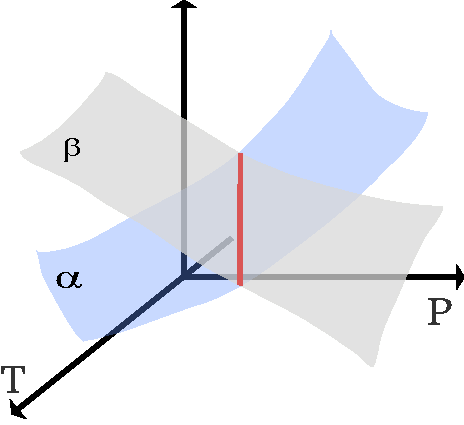
\includegraphics[width=0.8\textwidth]{../lessons/2_image/1.pdf}
\caption{\label{fig:2_1} Phase diagram: stability of phases.}
\end{figure}



To fix the ideas, let us choose a given value of pressure \( P = P^* \) and study the behaviour of \( g(T,P^*) \) as a function of \emph{T} when we go from solid to gas, as illustrated in Figure \ref{fig:2_2}.

\begin{figure}[h!]
\centering
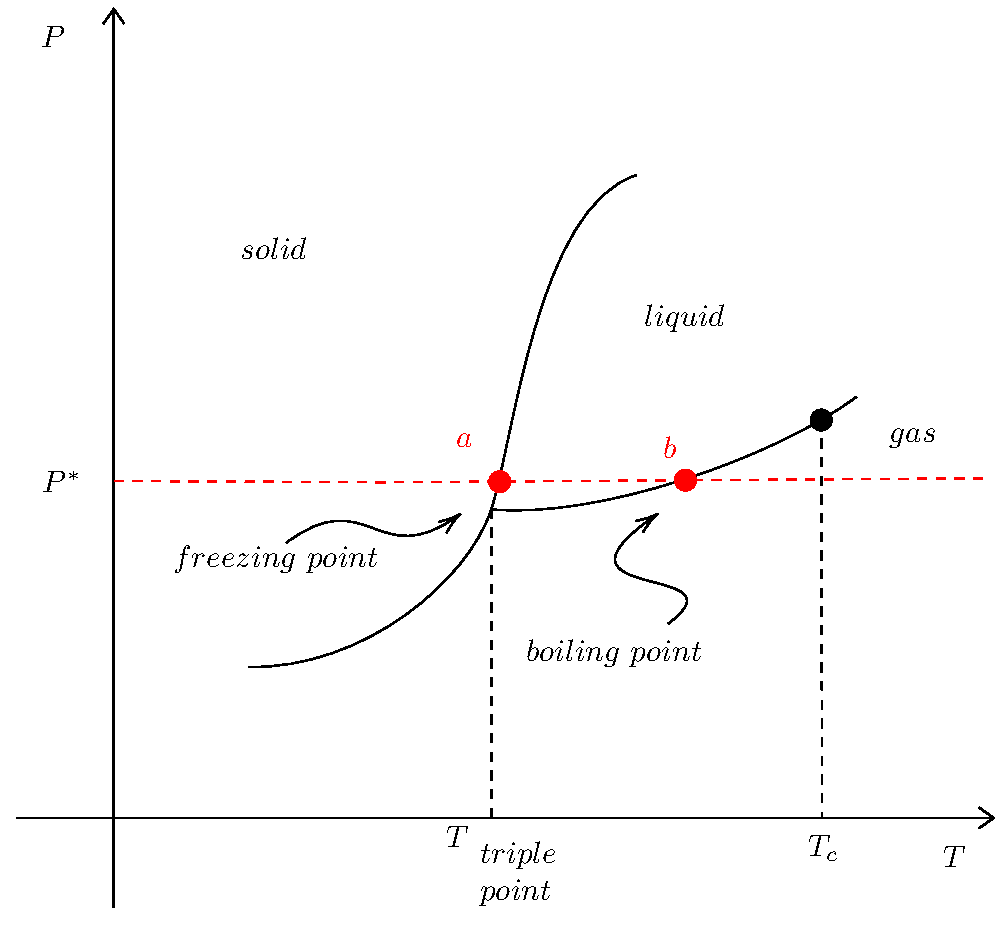
\includegraphics[width=0.75\textwidth]{../lessons/2_image/2.pdf}
\caption{\label{fig:2_2} \( (T,P) \) projection.}
\end{figure}



\begin{figure}[h!]
\centering
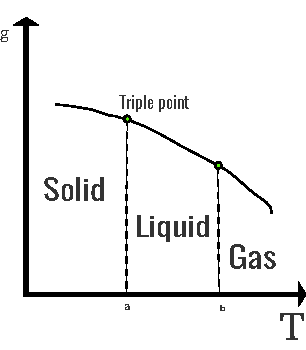
\includegraphics[width=0.62\textwidth]{../lessons/2_image/3.pdf}
\caption{\label{fig:2_3}  \( (g,T) \) projection at a fixed pression \( P = P^* \).}
\end{figure}

At the triple point \( g_{\text{solid}}(T_ a, P^*) = g_{\text{liq}}(T_a) \) and \( g_{\text{liq}}(T_b) = g_{\text{gas}}(T_b , P^*) \), as shown in Figure \ref{fig:2_3}.
Note also that:
\begin{itemize}
\item At the coexistence points \emph{a} and \emph{b} of the two phases, one has \( g_ \alpha (T) = g_ \beta (T) \).
\item \( g(T) \) is a continuous function of \emph{T}.
\item Note that, \( S= -\qty(\pdv{G}{T} )_V  \)  and \( c_P = - T \qty(\pdv[2]{G}{T}) > 0 \). This implies that \( g(T) \) is concave in \emph{T} at fixed \emph{P}.
\end{itemize}

\noindent
How about its derivatives? Since \emph{P}  is fixed we can vary \emph{T}  and look for \( s=-\qty(\pdv{g}{T} )_P  \). As we cross different phases  we have discontinuities, where \( \Delta s T \)  is called the \emph{latent heat}. It is illustrated in Figure \ref{fig:2_4}.



\begin{figure}[h!]
\centering
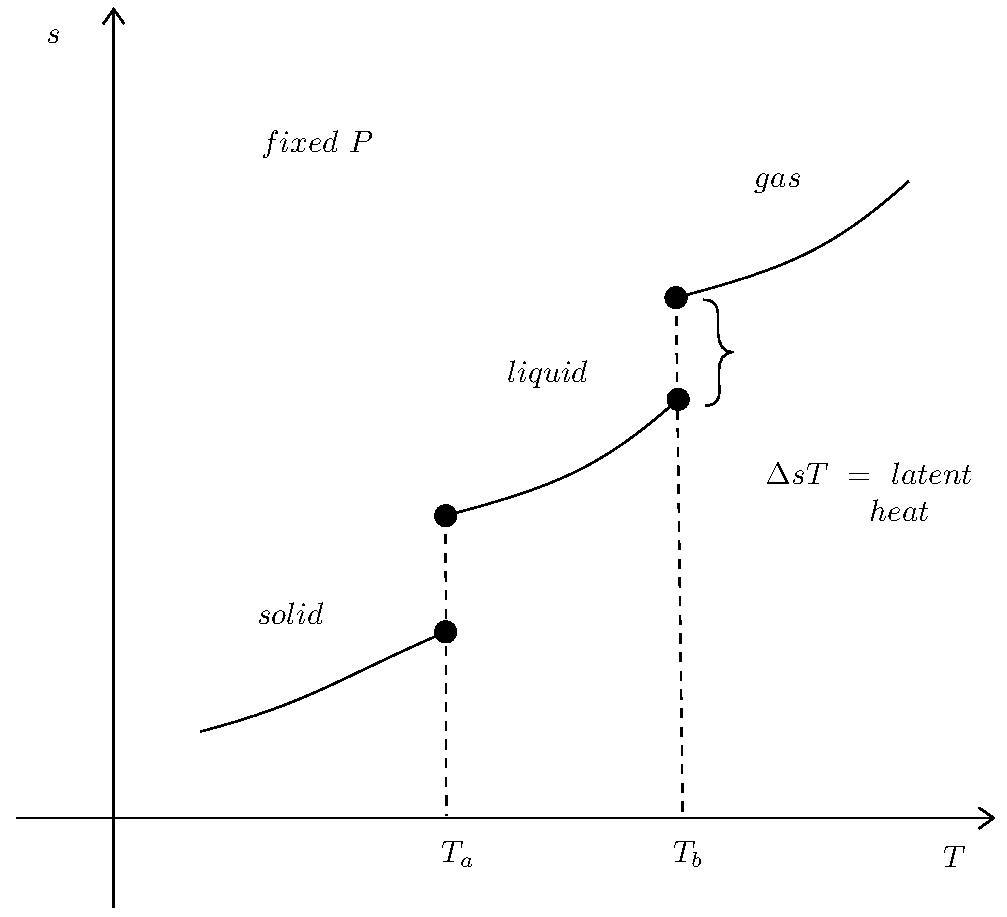
\includegraphics[width=0.62\textwidth]{../lessons/2_image/4.pdf}
\caption{\label{fig:2_4} \( (s,T) \) projection. }
\end{figure}


We can also fix the temperature \( T=T^* \)  and look at the variation of \emph{P}, as shown in Figure \ref{fig:2_5}.

\begin{figure}[h!]
\centering
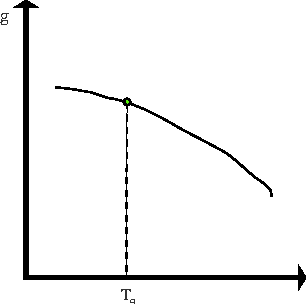
\includegraphics[width=1\textwidth]{../lessons/2_image/5.pdf}
\caption{\label{fig:2_5} Left: \( (T,P) \) projection. Right:  \( (g,P) \) projection at a fixed temperature \( T = T^* \).}
\end{figure}

\noindent
Note that, we have  \( v= \qty(\pdv{g}{P} )_T > 0  \) :
\begin{equation}
  \qty(\pdv[2]{g}{P} ) = \qty(\pdv{U}{P} )_T = -v k_T < 0
  \label{eq:}
\end{equation}
It is illustrated in Figure \ref{fig:2_6}.


\begin{figure}[h!]
\centering
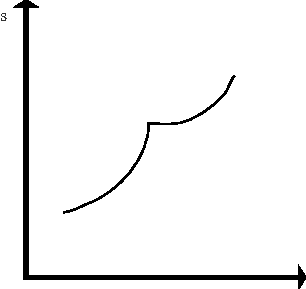
\includegraphics[width=0.7\textwidth]{../lessons/2_image/6.pdf}
\caption{\label{fig:2_6} \( (v,P) \) projection.}
\end{figure}



\section{Second order phase transition}
There are other cases in which we do not have these effects, as in Figure \ref{fig:2_7}. This is different from the previous situation in which we had a jump:
\begin{subequations}
\begin{align}
  \qty(\pdv{g}{T} )_P &= -s \\
  \qty(\pdv{g}{P} )_T &= v
\end{align}
\end{subequations}
they are continuous. However, this implies:
\begin{equation}
  \qty(\pdv{g}{T}{P}  ) = \qty(\pdv{v}{T} )_P = v_{\alpha p}
  \label{eq:}
\end{equation}
that is discontinuous.
An example is \emph{superconductivity}.


\begin{figure}[h!]
\begin{minipage}[c]{0.5\linewidth}
\centering
\subfloat[][Description]{


\tikzset{every picture/.style={line width=0.75pt}} %set default line width to 0.75pt

\begin{tikzpicture}[x=0.75pt,y=0.75pt,yscale=-0.4,xscale=0.4]
%uncomment if require: \path (0,433); %set diagram left start at 0, and has height of 433

%Shape: Axis 2D [id:dp34042133393206886]
\draw  (72,390.7) -- (543,390.7)(119.1,1) -- (119.1,434) (536,385.7) -- (543,390.7) -- (536,395.7) (114.1,8) -- (119.1,1) -- (124.1,8)  ;
%Straight Lines [id:da6702336744569144]
\draw  [dash pattern={on 4.5pt off 4.5pt}]  (301,106) -- (303,391) ;


%Curve Lines [id:da832017125366147]
\draw    (178,78) .. controls (309,90) and (446,145) .. (470,309) ;


%Shape: Circle [id:dp6821519031317774]
\draw  [color={rgb, 255:red, 0; green, 0; blue, 0 }  ,draw opacity=1 ][fill={rgb, 255:red, 0; green, 0; blue, 0 }  ,fill opacity=1 ] (296.05,106) .. controls (296.05,103.26) and (298.26,101.05) .. (301,101.05) .. controls (303.74,101.05) and (305.95,103.26) .. (305.95,106) .. controls (305.95,108.74) and (303.74,110.95) .. (301,110.95) .. controls (298.26,110.95) and (296.05,108.74) .. (296.05,106) -- cycle ;

% Text Node
\draw (93,24) node   {$g$};
% Text Node
\draw (524,409) node   {$T$};
% Text Node
\draw (308,419) node   {$T_{a}$};


\end{tikzpicture}

    \label{fig:} }
\end{minipage}
\begin{minipage}[]{0.5\linewidth}
\centering
\subfloat[][Description]{


\tikzset{every picture/.style={line width=0.75pt}} %set default line width to 0.75pt

\begin{tikzpicture}[x=0.75pt,y=0.75pt,yscale=-0.4,xscale=0.4]
%uncomment if require: \path (0,433); %set diagram left start at 0, and has height of 433

%Shape: Axis 2D [id:dp34042133393206886]
\draw  (72,390.7) -- (543,390.7)(119.1,1) -- (119.1,434) (536,385.7) -- (543,390.7) -- (536,395.7) (114.1,8) -- (119.1,1) -- (124.1,8)  ;
%Straight Lines [id:da6702336744569144]
\draw  [dash pattern={on 4.5pt off 4.5pt}]  (301,169) -- (303,391) ;


%Curve Lines [id:da832017125366147]
\draw    (152,330) .. controls (234,314) and (270,266) .. (301,169) ;


%Shape: Circle [id:dp6821519031317774]
\draw  [color={rgb, 255:red, 0; green, 0; blue, 0 }  ,draw opacity=1 ][fill={rgb, 255:red, 0; green, 0; blue, 0 }  ,fill opacity=1 ] (296.05,169) .. controls (296.05,166.26) and (298.26,164.05) .. (301,164.05) .. controls (303.74,164.05) and (305.95,166.26) .. (305.95,169) .. controls (305.95,171.74) and (303.74,173.95) .. (301,173.95) .. controls (298.26,173.95) and (296.05,171.74) .. (296.05,169) -- cycle ;
%Straight Lines [id:da1662494918814228]
\draw    (301,169) -- (451,88) ;



% Text Node
\draw (93,24) node   {$s$};
% Text Node
\draw (524,409) node   {$T$};
% Text Node
\draw (308,419) node   {$T_{a}$};


\end{tikzpicture}

    \label{fig:} }
\end{minipage}
\\
\begin{minipage}[c]{0.5\linewidth}
\centering
\subfloat[][Description]{


\tikzset{every picture/.style={line width=0.75pt}} %set default line width to 0.75pt

\begin{tikzpicture}[x=0.75pt,y=0.75pt,yscale=-0.4,xscale=0.4]
%uncomment if require: \path (0,433); %set diagram left start at 0, and has height of 433

%Shape: Axis 2D [id:dp34042133393206886]
\draw  (72,390.7) -- (543,390.7)(119.1,1) -- (119.1,434) (536,385.7) -- (543,390.7) -- (536,395.7) (114.1,8) -- (119.1,1) -- (124.1,8)  ;
%Straight Lines [id:da6702336744569144]
\draw  [dash pattern={on 4.5pt off 4.5pt}]  (301,169) -- (303,391) ;


%Shape: Circle [id:dp6821519031317774]
\draw  [color={rgb, 255:red, 0; green, 0; blue, 0 }  ,draw opacity=1 ][fill={rgb, 255:red, 0; green, 0; blue, 0 }  ,fill opacity=1 ] (296.05,169) .. controls (296.05,166.26) and (298.26,164.05) .. (301,164.05) .. controls (303.74,164.05) and (305.95,166.26) .. (305.95,169) .. controls (305.95,171.74) and (303.74,173.95) .. (301,173.95) .. controls (298.26,173.95) and (296.05,171.74) .. (296.05,169) -- cycle ;
%Straight Lines [id:da1662494918814228]
\draw    (301,169) -- (451,88) ;


%Straight Lines [id:da8938048927675745]
\draw    (301,169) -- (191,331) ;



% Text Node
\draw (93,24) node   {$v$};
% Text Node
\draw (524,409) node   {$P$};
% Text Node
\draw (308,419) node   {$T_{a}$};


\end{tikzpicture}

    \label{fig:} }
\end{minipage}
\begin{minipage}[]{0.5\linewidth}
\centering
\subfloat[][Description]{


\tikzset{every picture/.style={line width=0.75pt}} %set default line width to 0.75pt

\begin{tikzpicture}[x=0.75pt,y=0.75pt,yscale=-0.4,xscale=0.4]
%uncomment if require: \path (0,433); %set diagram left start at 0, and has height of 433

%Shape: Axis 2D [id:dp34042133393206886]
\draw  (72,390.7) -- (543,390.7)(119.1,1) -- (119.1,434) (536,385.7) -- (543,390.7) -- (536,395.7) (114.1,8) -- (119.1,1) -- (124.1,8)  ;
%Straight Lines [id:da6702336744569144]
\draw  [dash pattern={on 4.5pt off 4.5pt}]  (300,102) -- (303,391) ;


%Shape: Circle [id:dp6821519031317774]
\draw  [color={rgb, 255:red, 0; green, 0; blue, 0 }  ,draw opacity=1 ][fill={rgb, 255:red, 0; green, 0; blue, 0 }  ,fill opacity=1 ] (295.05,106.95) .. controls (295.05,104.22) and (297.26,102) .. (300,102) .. controls (302.74,102) and (304.95,104.22) .. (304.95,106.95) .. controls (304.95,109.69) and (302.74,111.91) .. (300,111.91) .. controls (297.26,111.91) and (295.05,109.69) .. (295.05,106.95) -- cycle ;
%Straight Lines [id:da1662494918814228]
\draw    (303,293) -- (453,212) ;


%Curve Lines [id:da3323852489584005]
\draw    (153,262) .. controls (198,248) and (293,190) .. (300,102) ;



% Text Node
\draw (93,24) node   {$c_{P}$};
% Text Node
\draw (524,409) node   {$T$};
% Text Node
\draw (308,419) node   {$T_{a}$};


\end{tikzpicture}

    \label{fig:2_7_4} }
\end{minipage}
\caption{\label{fig:2_7} Description}
\end{figure}

If we look for example at the specific heat in Figure \ref{fig:2_7_4}, it represent the transition from superconduction.

The critical point is special beacause there is not a jump, so we can go continuously from gas to liquid. The response function when we plot this point shows that the specific heat diverges.

The transitions are classified in the first order transition and continuous transition. The superfluid transition is a transition where the second derivative of the thermodynamic potential diverges. There are many phase transitions that can be classified in different ways.
We note that at the coexistence line we increase V, but the pression remains constant. At the coexistence line we see bubbles. It is the density that is changing locally, the bubbles becames bigger and bigger and at the \( V_G \) , becames a liquid.


\subsection{Helmholtz free-energy}
Consider \( A = A (T,V,N) \), here \emph{P} is replaced by \emph{V} which is discontinuous at the first order transition. Moreover \( P > 0 \)  implies \( \partial{A}/\partial{V} < 0   \) and
\begin{equation}
  k_T = -\frac{1}{V} \qty(\pdv{V}{P} )_T = -\frac{1}{V} \qty(\pdv{P}{V} )_T = \frac{1}{V} \qty(\pdv[2]{A}{V} )_T > 0
  \label{eq:}
\end{equation}
\emph{A} is an overall convex function of \emph{V}.
The behaviour of \emph{A} when there is a first order phase transition is as in Figure \ref{fig:2_8_1}. The linear sector becomes an horizontal one in the \( P = - (\partial{A}/\partial{V}  )_T = P (V) \) curve (Figure \ref{fig:2_8_2}).




\begin{figure}[h!]
\begin{minipage}[c]{0.5\linewidth}
\centering
\subfloat[][Description]{


\tikzset{every picture/.style={line width=0.75pt}} %set default line width to 0.75pt

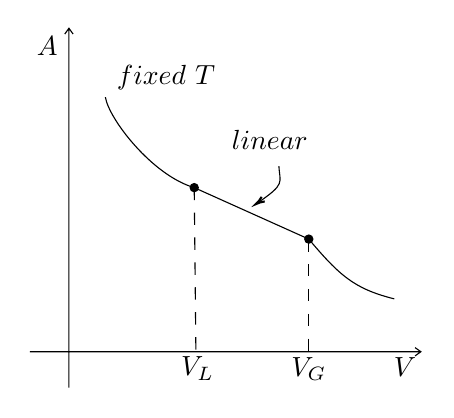
\begin{tikzpicture}[x=0.75pt,y=0.75pt,yscale=-0.4,xscale=0.4]
%uncomment if require: \path (0,433); %set diagram left start at 0, and has height of 433

%Shape: Axis 2D [id:dp34042133393206886]
\draw  (72,390.7) -- (543,390.7)(119.1,1) -- (119.1,434) (536,385.7) -- (543,390.7) -- (536,395.7) (114.1,8) -- (119.1,1) -- (124.1,8)  ;
%Straight Lines [id:da6702336744569144]
\draw  [dash pattern={on 4.5pt off 4.5pt}]  (270,193) -- (272,390) ;


%Shape: Circle [id:dp6821519031317774]
\draw  [color={rgb, 255:red, 0; green, 0; blue, 0 }  ,draw opacity=1 ][fill={rgb, 255:red, 0; green, 0; blue, 0 }  ,fill opacity=1 ] (265.05,193) .. controls (265.05,190.26) and (267.26,188.05) .. (270,188.05) .. controls (272.74,188.05) and (274.95,190.26) .. (274.95,193) .. controls (274.95,195.74) and (272.74,197.95) .. (270,197.95) .. controls (267.26,197.95) and (265.05,195.74) .. (265.05,193) -- cycle ;
%Straight Lines [id:da1662494918814228]
\draw    (270,193) -- (408,255) ;


%Straight Lines [id:da7053989083670136]
\draw  [dash pattern={on 4.5pt off 4.5pt}]  (408,255) -- (408,391) ;


%Curve Lines [id:da6886563534922254]
\draw    (408,255) .. controls (445,299) and (463,315) .. (511,327) ;


%Curve Lines [id:da48601947297403236]
\draw    (163,84) .. controls (167,110) and (219,178) .. (270,193) ;


%Shape: Circle [id:dp988494671197904]
\draw  [color={rgb, 255:red, 0; green, 0; blue, 0 }  ,draw opacity=1 ][fill={rgb, 255:red, 0; green, 0; blue, 0 }  ,fill opacity=1 ] (403.05,255) .. controls (403.05,252.26) and (405.26,250.05) .. (408,250.05) .. controls (410.74,250.05) and (412.95,252.26) .. (412.95,255) .. controls (412.95,257.74) and (410.74,259.95) .. (408,259.95) .. controls (405.26,259.95) and (403.05,257.74) .. (403.05,255) -- cycle ;
%Curve Lines [id:da30431708024345916]
\draw    (372,167) .. controls (372.99,187.69) and (380.76,188) .. (345.63,211.89) ;
\draw [shift={(344,213)}, rotate = 325.95] [color={rgb, 255:red, 0; green, 0; blue, 0 }  ][line width=0.75]    (10.93,-3.29) .. controls (6.95,-1.4) and (3.31,-0.3) .. (0,0) .. controls (3.31,0.3) and (6.95,1.4) .. (10.93,3.29)   ;


% Text Node
\draw (93,23) node   {$A$};
% Text Node
\draw (524,409) node   {$V$};
% Text Node
\draw (274,411) node   {$V_{L}$};
% Text Node
\draw (408,412) node   {$V_{G}$};
% Text Node
\draw (361,135) node   {$linear$};
% Text Node
\draw (236,60) node   {$fixed\ T$};


\end{tikzpicture}

    \label{fig:2_8_1} }
\end{minipage}
\begin{minipage}[]{0.5\linewidth}
\centering
\subfloat[][Description]{


\tikzset{every picture/.style={line width=0.75pt}} %set default line width to 0.75pt

\begin{tikzpicture}[x=0.75pt,y=0.75pt,yscale=-0.4,xscale=0.4]
%uncomment if require: \path (0,433); %set diagram left start at 0, and has height of 433

%Shape: Axis 2D [id:dp34042133393206886]
\draw  (72,390.7) -- (543,390.7)(119.1,1) -- (119.1,434) (536,385.7) -- (543,390.7) -- (536,395.7) (114.1,8) -- (119.1,1) -- (124.1,8)  ;
%Straight Lines [id:da6702336744569144]
\draw  [dash pattern={on 4.5pt off 4.5pt}]  (272,254) -- (272,390) ;


%Shape: Circle [id:dp6821519031317774]
\draw  [color={rgb, 255:red, 0; green, 0; blue, 0 }  ,draw opacity=1 ][fill={rgb, 255:red, 0; green, 0; blue, 0 }  ,fill opacity=1 ] (267.05,254) .. controls (267.05,251.26) and (269.26,249.05) .. (272,249.05) .. controls (274.74,249.05) and (276.95,251.26) .. (276.95,254) .. controls (276.95,256.74) and (274.74,258.95) .. (272,258.95) .. controls (269.26,258.95) and (267.05,256.74) .. (267.05,254) -- cycle ;
%Straight Lines [id:da1662494918814228]
\draw    (272,254) -- (408,255) ;


%Straight Lines [id:da7053989083670136]
\draw  [dash pattern={on 4.5pt off 4.5pt}]  (408,255) -- (408,391) ;


%Curve Lines [id:da6886563534922254]
\draw    (408,255) .. controls (445,299) and (463,315) .. (511,327) ;


%Curve Lines [id:da48601947297403236]
\draw    (165,145) .. controls (169,171) and (221,239) .. (272,254) ;


%Shape: Circle [id:dp988494671197904]
\draw  [color={rgb, 255:red, 0; green, 0; blue, 0 }  ,draw opacity=1 ][fill={rgb, 255:red, 0; green, 0; blue, 0 }  ,fill opacity=1 ] (403.05,255) .. controls (403.05,252.26) and (405.26,250.05) .. (408,250.05) .. controls (410.74,250.05) and (412.95,252.26) .. (412.95,255) .. controls (412.95,257.74) and (410.74,259.95) .. (408,259.95) .. controls (405.26,259.95) and (403.05,257.74) .. (403.05,255) -- cycle ;

% Text Node
\draw (93,23) node   {$P$};
% Text Node
\draw (524,409) node   {$V$};
% Text Node
\draw (274,411) node   {$V_{L}$};
% Text Node
\draw (408,412) node   {$V_{G}$};


\end{tikzpicture}

    \label{fig:2_8_2} }
\end{minipage}
\caption{\label{fig:2_8} Description}
\end{figure}



\subsection{Critical points}
At the critical point \( (P_c,T_c) \) the system can pass from the liquid to the gas phase (and viceversa) in a continuous way
\begin{equation}
  \Delta s = \Delta v = 0
  \label{eq:}
\end{equation}
Usually critical points are end point of first order transition phases. Why there is no critical point between solid and liquid? The crossover between phases having the same symmetry define the Landau point. There is a break of symmetry, for instance we can think about the structure of the bravais lattice. Instead, from gas to liquid symmetries are not broken.

\begin{figure}[h!]
\centering


\tikzset{every picture/.style={line width=0.75pt}} %set default line width to 0.75pt

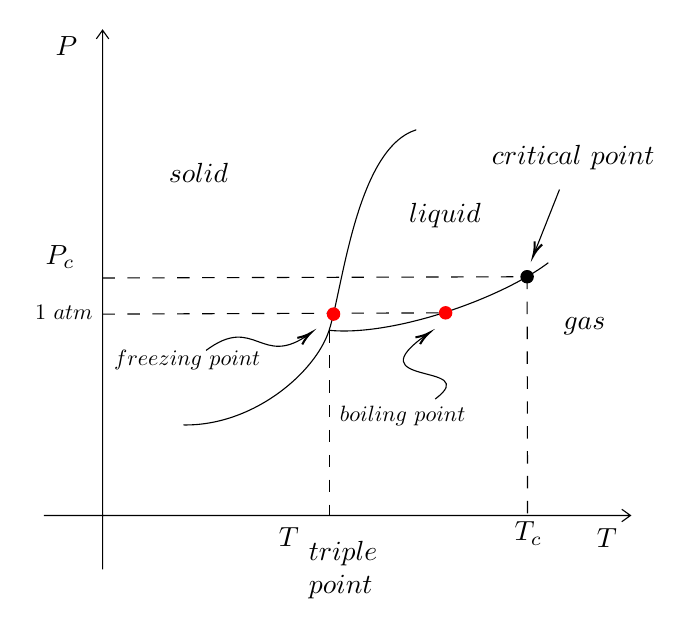
\begin{tikzpicture}[x=0.75pt,y=0.75pt,yscale=-0.6,xscale=0.6]
%uncomment if require: \path (0,433); %set diagram left start at 0, and has height of 433

%Shape: Axis 2D [id:dp34042133393206886]
\draw  (72,390.7) -- (543,390.7)(119.1,1) -- (119.1,434) (536,385.7) -- (543,390.7) -- (536,395.7) (114.1,8) -- (119.1,1) -- (124.1,8)  ;
%Curve Lines [id:da2649058921866929]
\draw    (184,318) .. controls (240,319) and (290,276) .. (301,242) .. controls (312,208) and (323,96) .. (371,81) ;


%Curve Lines [id:da19336772925785306]
\draw    (301,242) .. controls (351,247) and (437.06,217.73) .. (477.06,187.73) ;


%Straight Lines [id:da1379576233427211]
\draw  [dash pattern={on 4.5pt off 4.5pt}]  (301,242) -- (301,390) ;


%Straight Lines [id:da6702336744569144]
\draw  [dash pattern={on 4.5pt off 4.5pt}]  (460,199) -- (460.35,390.47) ;


%Shape: Circle [id:dp768993062031393]
\draw  [color={rgb, 255:red, 255; green, 0; blue, 0 }  ,draw opacity=1 ][fill={rgb, 255:red, 255; green, 0; blue, 0 }  ,fill opacity=1 ] (389.6,227.98) .. controls (389.6,225.24) and (391.82,223.03) .. (394.55,223.03) .. controls (397.29,223.03) and (399.51,225.24) .. (399.51,227.98) .. controls (399.51,230.72) and (397.29,232.93) .. (394.55,232.93) .. controls (391.82,232.93) and (389.6,230.72) .. (389.6,227.98) -- cycle ;
%Curve Lines [id:da897292552339868]
\draw    (202.21,258.16) .. controls (241.81,228.46) and (246.13,273.25) .. (285.02,245.04) ;
\draw [shift={(286.21,244.16)}, rotate = 503.13] [color={rgb, 255:red, 0; green, 0; blue, 0 }  ][line width=0.75]    (10.93,-3.29) .. controls (6.95,-1.4) and (3.31,-0.3) .. (0,0) .. controls (3.31,0.3) and (6.95,1.4) .. (10.93,3.29)   ;

%Curve Lines [id:da43687585409049334]
\draw    (386.21,297.16) .. controls (426.01,267.31) and (318.3,287.95) .. (380.27,244.82) ;
\draw [shift={(381.21,244.16)}, rotate = 505.49] [color={rgb, 255:red, 0; green, 0; blue, 0 }  ][line width=0.75]    (10.93,-3.29) .. controls (6.95,-1.4) and (3.31,-0.3) .. (0,0) .. controls (3.31,0.3) and (6.95,1.4) .. (10.93,3.29)   ;

%Shape: Circle [id:dp07400034471483774]
\draw  [color={rgb, 255:red, 0; green, 0; blue, 0 }  ,draw opacity=1 ][fill={rgb, 255:red, 0; green, 0; blue, 0 }  ,fill opacity=1 ] (455.05,199) .. controls (455.05,196.26) and (457.26,194.05) .. (460,194.05) .. controls (462.74,194.05) and (464.95,196.26) .. (464.95,199) .. controls (464.95,201.74) and (462.74,203.95) .. (460,203.95) .. controls (457.26,203.95) and (455.05,201.74) .. (455.05,199) -- cycle ;
%Straight Lines [id:da29969851398494274]
\draw  [dash pattern={on 4.5pt off 4.5pt}]  (119,200) -- (460,199) ;


%Straight Lines [id:da602287698180992]
\draw  [dash pattern={on 4.5pt off 4.5pt}]  (119,229) -- (394.55,227.98) ;


%Shape: Circle [id:dp4330038061237751]
\draw  [color={rgb, 255:red, 255; green, 0; blue, 0 }  ,draw opacity=1 ][fill={rgb, 255:red, 255; green, 0; blue, 0 }  ,fill opacity=1 ] (299.6,228.98) .. controls (299.6,226.24) and (301.82,224.03) .. (304.55,224.03) .. controls (307.29,224.03) and (309.51,226.24) .. (309.51,228.98) .. controls (309.51,231.72) and (307.29,233.93) .. (304.55,233.93) .. controls (301.82,233.93) and (299.6,231.72) .. (299.6,228.98) -- cycle ;
%Straight Lines [id:da2746826747815124]
\draw    (486,129) -- (465.74,180.14) ;
\draw [shift={(465,182)}, rotate = 291.61] [color={rgb, 255:red, 0; green, 0; blue, 0 }  ][line width=0.75]    (10.93,-3.29) .. controls (6.95,-1.4) and (3.31,-0.3) .. (0,0) .. controls (3.31,0.3) and (6.95,1.4) .. (10.93,3.29)   ;


% Text Node
\draw (196,116) node   {$solid$};
% Text Node
\draw (394,150) node   {$liquid$};
% Text Node
\draw (506,239) node   {$gas$};
% Text Node
\draw (187,266.16) node [scale=0.8] {$freezing\ point$};
% Text Node
\draw (360,311.16) node  [scale=0.8] {$boiling\ point$};
% Text Node
\draw (310,431.16) node   {$T_{ \begin{array}{l}
triple\ \\
point
\end{array}}$};
% Text Node
\draw (461,405.16) node   {$T_{c}$};
% Text Node
\draw (90,14) node   {$P$};
% Text Node
\draw (524,409) node   {$T$};
% Text Node
\draw (497,103) node   {$critical\ point$};
% Text Node
\draw (88,228) node  [scale=0.8] {$1\ atm$};
% Text Node
\draw (85,183) node   {$P_{c}$};


\end{tikzpicture}

\caption{\label{fig:2_9} Description.}
\end{figure}



\subsection{Ferromagnetic system}



\begin{figure}[h!]
\centering


\tikzset{every picture/.style={line width=0.75pt}} %set default line width to 0.75pt

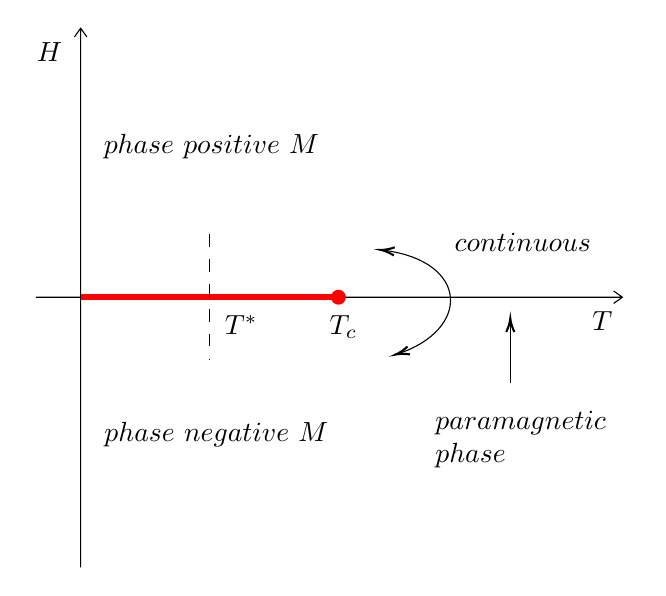
\begin{tikzpicture}[x=0.75pt,y=0.75pt,yscale=-0.6,xscale=0.6]
%uncomment if require: \path (0,433); %set diagram left start at 0, and has height of 433

%Shape: Axis 2D [id:dp34042133393206886]
\draw  (72,217) -- (543,217)(108,1) -- (108,434) (536,212) -- (543,217) -- (536,222) (103,8) -- (108,1) -- (113,8)  ;
%Straight Lines [id:da9551803962585098]
\draw [color={rgb, 255:red, 255; green, 0; blue, 0 }  ,draw opacity=1 ][line width=2.25]    (108,217) -- (315,217) ;


%Shape: Circle [id:dp40105900325823207]
\draw  [color={rgb, 255:red, 255; green, 0; blue, 0 }  ,draw opacity=1 ][fill={rgb, 255:red, 255; green, 0; blue, 0 }  ,fill opacity=1 ] (309.48,217) .. controls (309.48,213.95) and (311.95,211.48) .. (315,211.48) .. controls (318.05,211.48) and (320.52,213.95) .. (320.52,217) .. controls (320.52,220.05) and (318.05,222.52) .. (315,222.52) .. controls (311.95,222.52) and (309.48,220.05) .. (309.48,217) -- cycle ;
%Curve Lines [id:da3888044898644526]
\draw    (351.14,179.25) .. controls (420.32,188.05) and (421.38,243.07) .. (362.79,262.42) ;
\draw [shift={(361,263)}, rotate = 342.7] [color={rgb, 255:red, 0; green, 0; blue, 0 }  ][line width=0.75]    (10.93,-3.29) .. controls (6.95,-1.4) and (3.31,-0.3) .. (0,0) .. controls (3.31,0.3) and (6.95,1.4) .. (10.93,3.29)   ;
\draw [shift={(349,179)}, rotate = 6.34] [color={rgb, 255:red, 0; green, 0; blue, 0 }  ][line width=0.75]    (10.93,-3.29) .. controls (6.95,-1.4) and (3.31,-0.3) .. (0,0) .. controls (3.31,0.3) and (6.95,1.4) .. (10.93,3.29)   ;
%Straight Lines [id:da7184186969465476]
\draw  [dash pattern={on 4.5pt off 4.5pt}]  (211.5,166.5) -- (211.5,267.5) ;


%Straight Lines [id:da6340484806973028]
\draw    (453,286) -- (453,236) ;
\draw [shift={(453,234)}, rotate = 450] [color={rgb, 255:red, 0; green, 0; blue, 0 }  ][line width=0.75]    (10.93,-3.29) .. controls (6.95,-1.4) and (3.31,-0.3) .. (0,0) .. controls (3.31,0.3) and (6.95,1.4) .. (10.93,3.29)   ;


% Text Node
\draw (83,20) node   {$H$};
% Text Node
\draw (527,236) node   {$T$};
% Text Node
\draw (319,241) node   {$T_{c}$};
% Text Node
\draw (463,173) node   {$continuous$};
% Text Node
\draw (237,239) node   {$T^{*}$};
% Text Node
\draw (213,96) node   {$phase\ positive\ M$};
% Text Node
\draw (217,327) node   {$phase\ negative\ M$};
% Text Node
\draw (465,331) node   {$ \begin{array}{l}
paramagnetic\ \\
phase
\end{array}$};


\end{tikzpicture}

\caption{\label{fig:2_10} Description.}
\end{figure}

We can have a magnetization different from 0 even when the is no magnetic field.
Supposing \( P \leftrightarrow H, V \leftrightarrow M \), we have \( (P,T) \leftrightarrow (H,T) \). We have two equilibrium states that are connected continuosly, this is a first order transition. For instance consider Figure \ref{fig:2_11}. At  the critical point the magnetization would pass through zero.


\begin{figure}[h!]
\centering


\tikzset{every picture/.style={line width=0.75pt}} %set default line width to 0.75pt

\begin{tikzpicture}[x=0.75pt,y=0.75pt,yscale=-0.6,xscale=0.6]
%uncomment if require: \path (0,433); %set diagram left start at 0, and has height of 433

%Shape: Axis 2D [id:dp34042133393206886]
\draw  (72,216) -- (543,216)(308,1) -- (308,434) (536,211) -- (543,216) -- (536,221) (303,8) -- (308,1) -- (313,8)  ;
%Curve Lines [id:da28812631348081497]
\draw    (307.52,140) .. controls (347.52,110) and (387.52,80) .. (471.52,94) ;


%Curve Lines [id:da9601274154107028]
\draw    (141,361) .. controls (206,365) and (266,343) .. (307,295) ;


%Shape: Circle [id:dp6424722409409431]
\draw  [color={rgb, 255:red, 255; green, 0; blue, 0 }  ,draw opacity=1 ][fill={rgb, 255:red, 255; green, 0; blue, 0 }  ,fill opacity=1 ] (301.48,295) .. controls (301.48,291.95) and (303.95,289.48) .. (307,289.48) .. controls (310.05,289.48) and (312.52,291.95) .. (312.52,295) .. controls (312.52,298.05) and (310.05,300.52) .. (307,300.52) .. controls (303.95,300.52) and (301.48,298.05) .. (301.48,295) -- cycle ;
%Shape: Circle [id:dp3899266908502126]
\draw  [color={rgb, 255:red, 255; green, 0; blue, 0 }  ,draw opacity=1 ][fill={rgb, 255:red, 255; green, 0; blue, 0 }  ,fill opacity=1 ] (302,140) .. controls (302,136.95) and (304.47,134.48) .. (307.52,134.48) .. controls (310.57,134.48) and (313.04,136.95) .. (313.04,140) .. controls (313.04,143.05) and (310.57,145.52) .. (307.52,145.52) .. controls (304.47,145.52) and (302,143.05) .. (302,140) -- cycle ;

% Text Node
\draw (260,21) node   {$< M >$};
% Text Node
\draw (528,237) node   {$H$};
% Text Node
\draw (167,86) node   {$T\ =\ T^{*} \ < \ Tc$};

\end{tikzpicture}

\caption{\label{fig:2_11} Description.}
\end{figure}




\end{document}
